\documentclass[18pts]{article}
\usepackage{amssymb,amsmath,latexsym,enumerate,graphicx,fullpage,url,multicol,longtable,color}
\usepackage{graphicx, tikz}
\usetikzlibrary{calc,shadows}
\usepackage[T1]{fontenc}
\usepackage{eso-pic,fancybox}
\usepackage[absolute,overlay]{textpos}
\usepackage{color}
\usepackage{mathptmx}
\usepackage{fix-cm}

%    \topmargin 0 in
%    \textheight 11in
%    \textwidth 6.25 in
%    \oddsidemargin 1in   % read Lamport p.163
%    \evensidemargin 1 in
%    \headsep = 20pt
\usepackage{anyfontsize}
\usepackage{xparse}

% suppresses hyphenation and aligns left
\usepackage[none]{hyphenat}
\raggedright


\newcommand\ProjectName[1]{
{
\fontsize{35}{40}\selectfont
\noindent\textbf{#1}\par
}
\vskip 2mm
\fontsize{20}{25}\selectfont
}

\newenvironment{justified}
{
\tolerance=1
\emergencystretch=\maxdimen
\hyphenpenalty=10000
\hbadness=10000
}


\renewcommand\large{
\noindent\fontsize{16}{19}\selectfont}
\renewcommand\Large{
\noindent\fontsize{18}{20}\selectfont}


%%%%%%%%%%%%%%%%%%%%%%%%%%%%%%%%%%%%%%%%%%%%%%%%%%%%%%
%
%					DO NOT CHANGE ANY ABOVE FORMAT/MACRO
%
%%%%%%%%%%%%%%%%%%%%%%%%%%%%%%%%%%%%%%%%%%%%%%%%%%%%%%
\begin{document}

\ProjectName{Automatic Theorem Proving}
\noindent\textbf{Faculty Mentor: {Professor Philipp Hieronymi}
}
\vskip 2mm
\noindent\textbf{Team Leader: {Christian Schulz}
}
\vskip 2mm
\noindent\textbf{Scholars: Reed Oei, Eric Ma, Tatum Schmidt, Abdullah Dean}
\\
\vskip 2mm
\Large

\begin{justified}
An \emph{automated theorem prover} is a program that takes as input a statement and \emph{decides} (i.e., proves or disproves) it. 
Theorem provers can be very useful: computers are reliable, and they never get tired or bored, allowing us to quickly explore new ideas.
Though it is impossible to decide \textbf{all} statements, we can still use theorem provers to solve many interesting problems.\vspace{2mm}

% I'd like to use \ref instead of hardcoding Figure 1/2, but it doesn't seem to work... :(
% Put label after caption https://www.overleaf.com/learn/latex/Referencing_Figures
This semester, our group developed a theorem prover, which we call Pecan (Figure \ref{fig:pecan}), that automatically decides logical statements expressed via B\"uchi automata, a simplified model of a computer that can handle infinitely long inputs. 
We hope to use Pecan to expand on prior work on \emph{Sturmian words} (Figure \ref{fig:slope}), and automatically prove theorems about all Sturmian words at once rather than only special classes of Sturmian words. 
\end{justified}

\vskip 4mm

\begin{figure}[h]
\begin{minipage}{.49\textwidth}
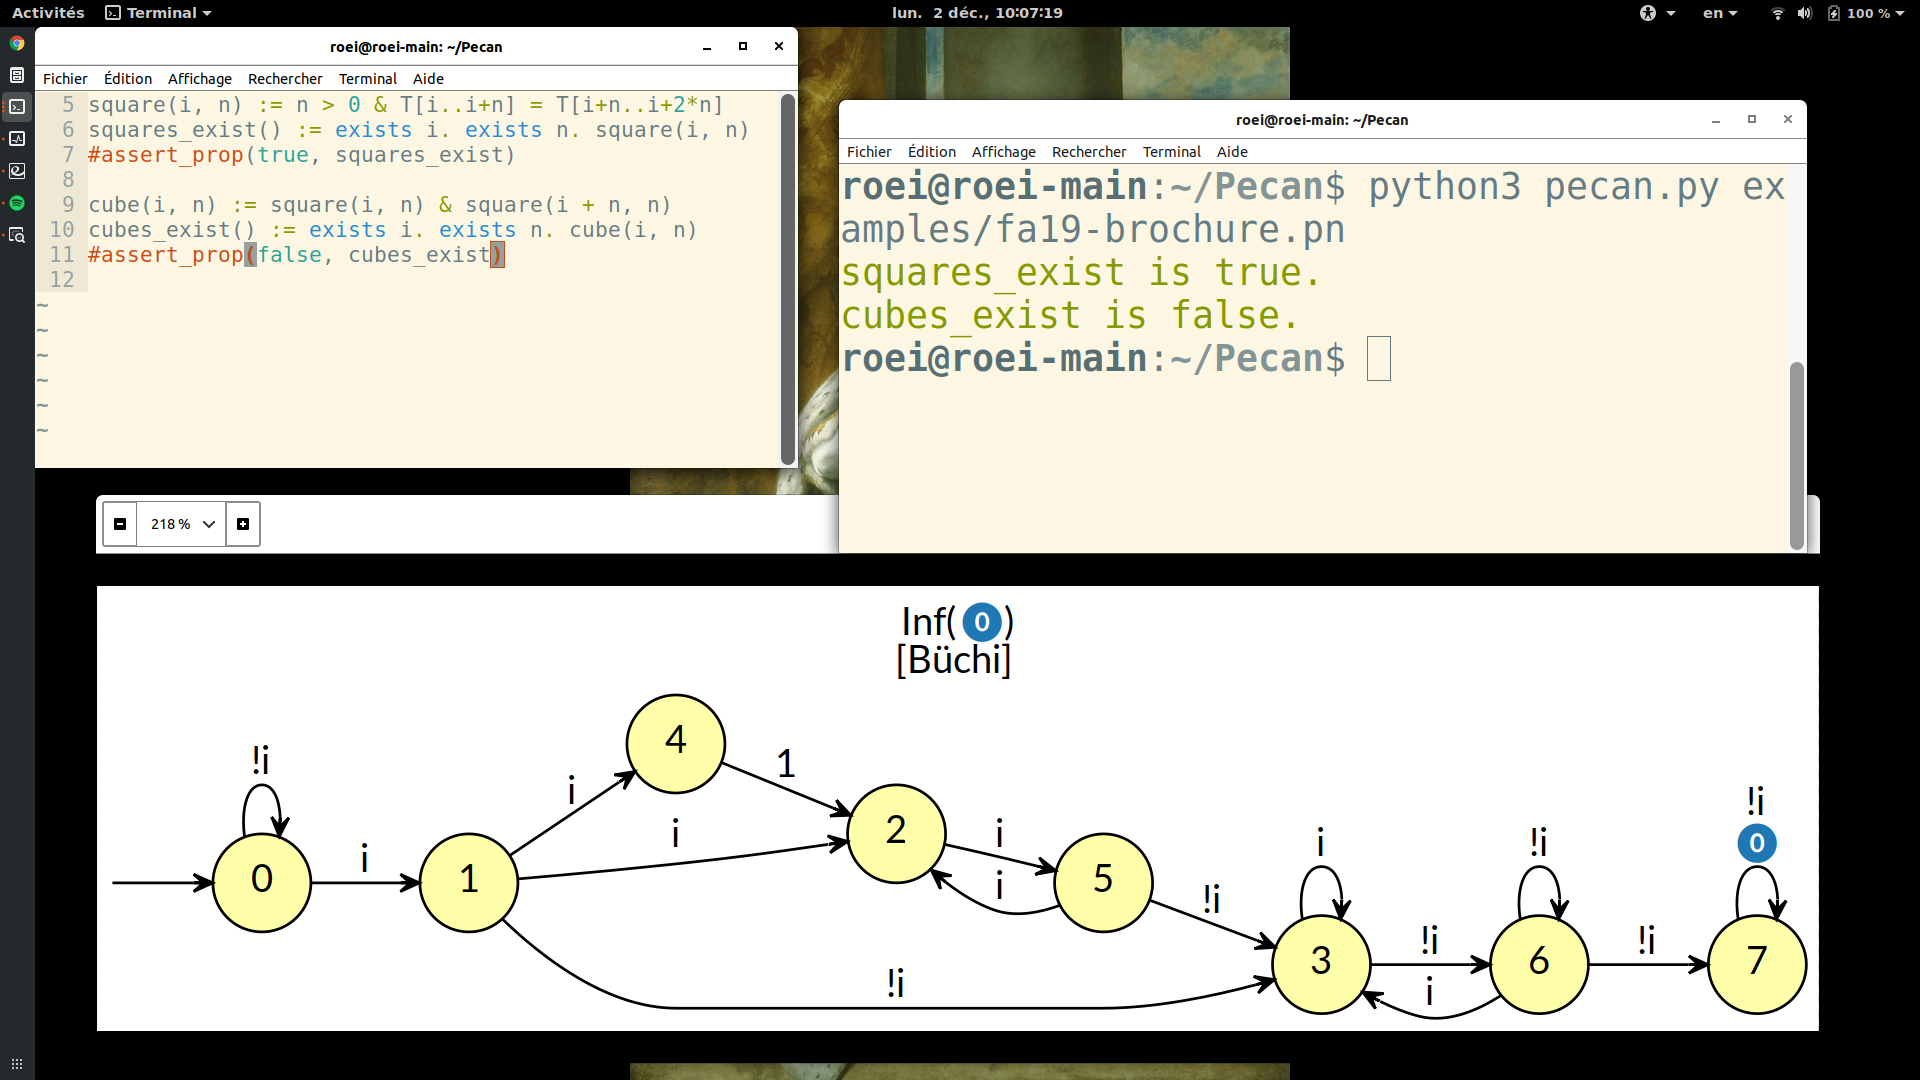
\includegraphics[width=\textwidth]{images/pecan-demo.png}%
\caption{A Pecan program and its output.}
\label{fig:pecan}
\end{minipage}
\hfill
\begin{minipage}{.49\textwidth}
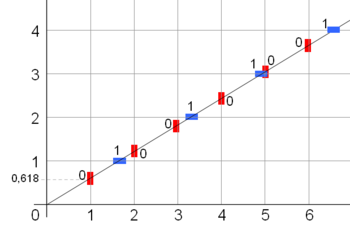
\includegraphics[width=\textwidth]{images/Fibonacci_word_cutting_sequence.png}%
\vspace{-6mm}
\caption{The Sturmian word with slope $1/\phi$, which starts with $0100101001\ldots$}
\label{fig:slope}
\end{minipage}
\end{figure}

\end{document}
